\chapter{Implementation}
\label{ch:implementation}

In this chapter the implementation is discussed, presenting how the objects are recognized and how the symbolic predicates are obtained. 

\section{Object Localization} 
For the planner, to know how to move the object, is fundamental knowing the objects on the scenario, therefore they need to be detected. More correctly, they need to be segmented since the algorithm is dealing with unknown objects, it is not going to recognize an objects as a particular one, but it segments the objects. 

This stage is composed on two steps:
\begin{enumerate}
\item Detecting the table top objects
\item Segmenting the table top objects
\end{enumerate}
The depth sensor is recording a depth map of a table, the algorithm has therefore to detect first the table, and so the objects that stands on top of it, and then segmenting them. We don't want to segment the entire image, if so, the table will be segmented as an object and the floor as well.

\subsection{Tabletop Object Detection} 
The strategy for the tabletop object detection phase is composed of 3 different steps:
\begin{enumerate}
\item \textbf{Table plane estimation} (by RANSAC): the points of the table are detected estimating first a plane in the point cloud, all the points which belong to such a plane are the points of the table. 
\item \textbf{2D Convex Hull of the table}: having the points of the table a 2D convex hull is computed in order to get a 2D shape containing those points.
\item \textbf{Polygonal prism projection}: all the points are projected on the table plane previously estimated and all the points which projections belong to the 2D convex hull are considered to be points of tabletop objects. 
\end{enumerate}

\begin{figure}[htp]
\centering
\begin{subfigure}[t]{0.32\textwidth}
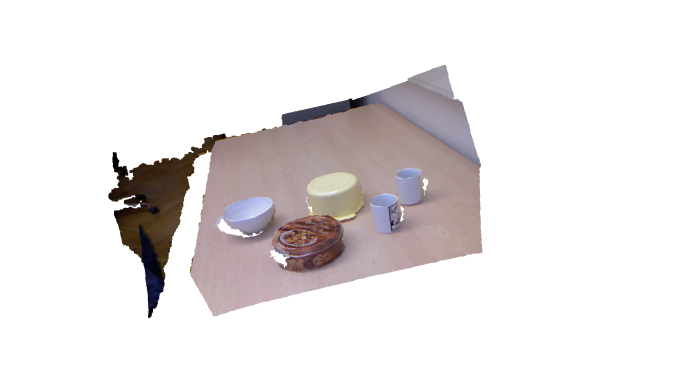
\includegraphics[width = 1.1\textwidth]{Img/ObjectSegmentation/pcl.png}
\caption{Input Point Cloud}\label{img:obj_pointcloud}
\end{subfigure}
\begin{subfigure}[t]{0.32\textwidth}
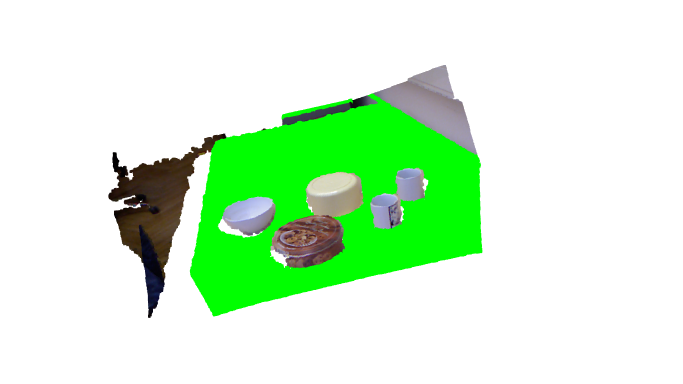
\includegraphics[width = 1.1\textwidth]{Img/ObjectSegmentation/ransac.png}
\caption{RANSAC plane estimation}\label{img:obj_ransac}
\end{subfigure}
\begin{subfigure}[t]{0.32\textwidth}
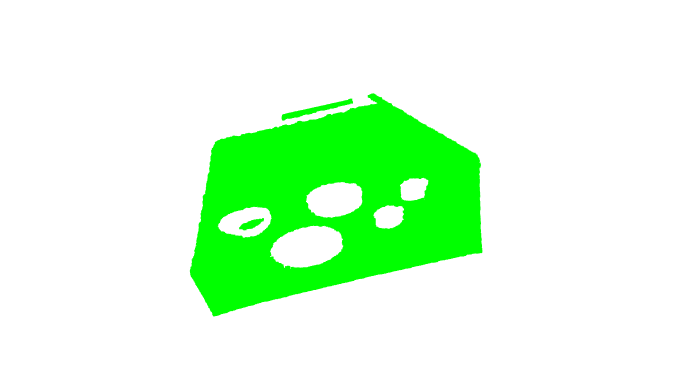
\includegraphics[width = 1.1\textwidth]{Img/ObjectSegmentation/plane.png}
\caption{Table plane}\label{img:obj_plane}
\end{subfigure}
\begin{subfigure}[t]{0.32\textwidth}
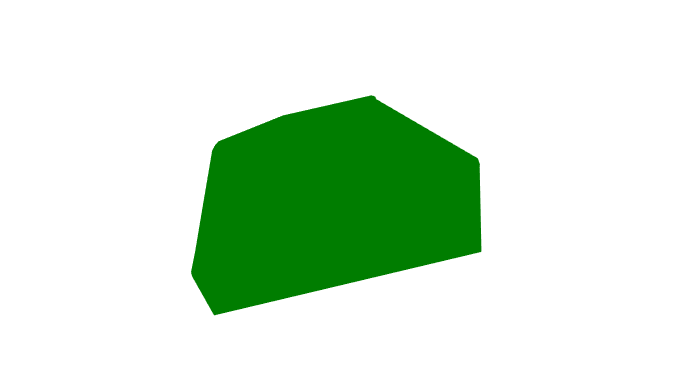
\includegraphics[width = 1.1\textwidth]{Img/ObjectSegmentation/convex_hull.png}
\caption{Convex Hull}\label{img:obj_conex_hull}
\end{subfigure}
\begin{subfigure}[t]{0.32\textwidth}
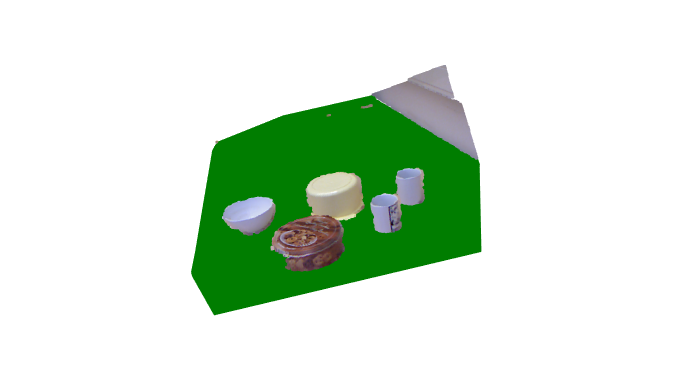
\includegraphics[width = 1.1\textwidth]{Img/ObjectSegmentation/convex_hull_full.png}
\caption{Convex hull in the point cloud}\label{img:obj_convex_hull_full}
\end{subfigure}
\begin{subfigure}[t]{0.32\textwidth}
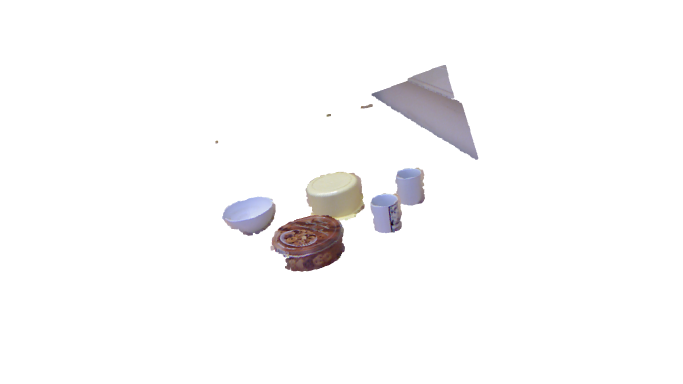
\includegraphics[width = 1.1\textwidth]{Img/ObjectSegmentation/tabletop_objects.png}
\caption{Tabletop objects}\label{img:obj_tabletop_objects_results}
\end{subfigure}
\caption{\textbf{Object Segmentation:} Given the point cloud (\subref{img:obj_pointcloud}), the estimated table's plane is obtained (\subref{img:obj_ransac} and \subref{img:obj_plane}), its convex hull is extracted (\subref{img:obj_conex_hull} and \subref{img:obj_convex_hull_full}), and the tabletop objects are obtained by a polygonal prism projection (\subref{img:obj_tabletop_objects_results}).}
\label{img:obj_tabletop_objects}
\end{figure}

The steps of this tabletop object detection algorithm are described in Figure \ref{img:obj_tabletop_objects}   for the point cloud\footnote{Point cloud taken from the Object Segmentation Database (OSD) \href{http://users.acin.tuwien.ac.at/arichtsfeld/?site=4}{http://users.acin.tuwien.ac.at/arichtsfeld/?site=4}} in Figure \ref{img:obj_pointcloud}.

\subsection{Object Segmentation}
\label{sec:obj_seg}
Once the objects on the table are detected the following phase is to segment them in order to get a point cloud per object.

\subsubsection{Supervoxel}

For their segmentation the supervoxel concept is used. A supervoxel is a group of voxels that share similar characteristics. 
%and it is equivalent to the superpixel concept for the voxel case. Superpixel is a widely used preprocessing step in segmentation
%algorithms  which allows to reduce the number of regions
%that must be considered later by more computationally
%expensive algorithms, with a minimal loss of information. 
%The supervoxel concept is the extension of the superpixel method to the point clouds. A voxel represents a single sample on a regularly spaced, three-dimensional grid. A supervoxel 

In this work the supervoxels are computed with the Voxel Cloud Connectivy Segmentation (\texttt{VCCS}) algorithm \cite{Papon13CVPR}, which was proposed in 2014 and gives good improvements with respect to previous state of the art methods, and still it is able to be used in online applications. 

The algorithm works in 4 main steps:
\begin{itemize}
\item Voxelizing the point cloud
\item Creating an adjacency graph for the voxel-cloud 
\item Creating seeds for the initial supervoxels centres
\item Each seed is described by $39$ features that describe spatial coordinates, colors and local surface model properties. Then a distance metric based on  these features is defined. 
\item Clustering the voxels into supervoxles iteratively by means of the distance metric, the adjacency graph, and the search volume of the supervoxel. 
\item Once the search of all supervoxel adjacency graphs has been concluded, the centres of each supervoxel is updated by taking the mean of all its constituents. 
\end{itemize} 

\subsubsection{Local Convex Connected Patches Segmentation}
\label{sec:LCCP}
Once the supervoxels of the objects are computed, they can be clustered in order to segment the objects. Papon et al. also proposed a segmentation algorithm based on their supervoxel technique, called \textit{Local Convex Connected Patches Segmentation} (\texttt{LCCP}) \citep{LCCP}. This algorithm permits to segment objects by clustering together adjacent convex supervoxels.  The algorithm is quite simple but very good for segmentation of objects that have convex shapes, in Figure \ref{img:LCCP_structure} the algorithm is briefly described. 

\begin{figure}[h]
\centering
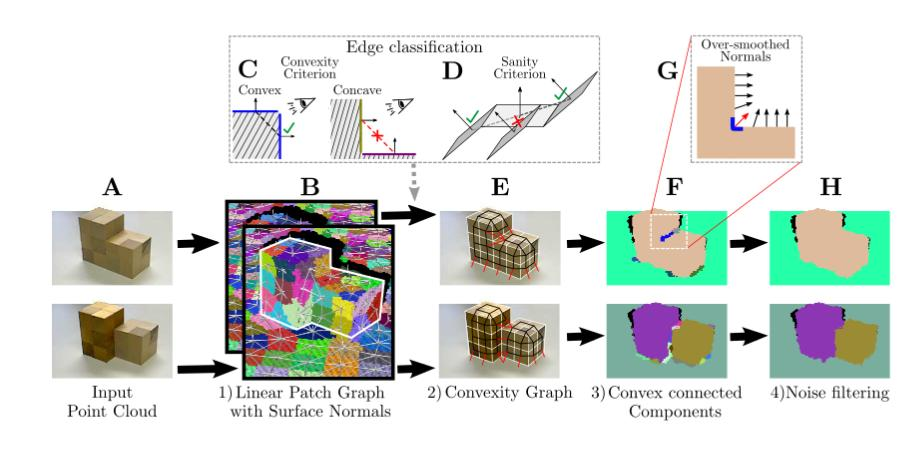
\includegraphics[width=\textwidth]{Img/ObjectSegmentation/lccp_structure.jpg}
\caption{\texttt{LCCP} algorithm's structure. Reproduced from \citep{LCCP}}
\label{img:LCCP_structure}
\end{figure}

It clusters all the adjacent convex supervoxels (patches) using two criterion:
\begin{itemize}
\item Extended criterion: to consider two adjacent patches convex, both must have a connection to a patch which is convex with respect both patches
\item Sanity Criterion: check if the adjacent patches which can be considered as convex present geometric discontinuities (see point D of Figure \ref{img:LCCP_structure}), in this case they are not considered as valid to form a cluster.
\end{itemize}
Then, due to the smoothed normals that could appear in some edges of the objects (point G Figure \ref{img:LCCP_structure}), the algorithm merges the clusters that are composed of few supervoxels to the biggest adjacent cluster. 

By tuning properly the parameters of the segmentation algorithm the objects can be correctly segmented obtaining for one of them a point cloud. Two examples of the segmentation algorithm for a cluttered scene are depicted in Figure \ref{fig:seg_results}. 

\begin{figure}[h]
\centering
\begin{subfigure}[t]{0.2\textwidth}
\centering
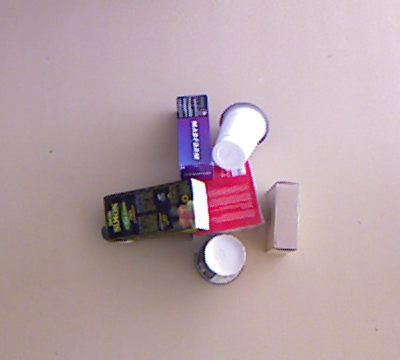
\includegraphics[width=\textwidth]{Img/ObjectSegmentation/seg1_rgb.png}
\end{subfigure}
\begin{subfigure}[t]{0.2\textwidth}
\centering
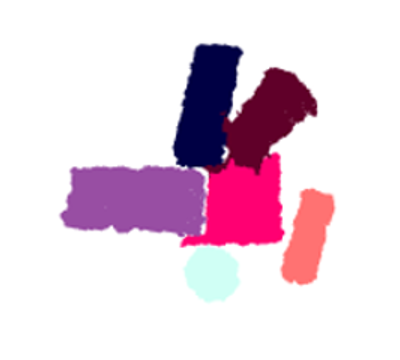
\includegraphics[width=\textwidth]{Img/ObjectSegmentation/seg1.png}
\end{subfigure}
\hspace{1.5cm}
\begin{subfigure}[t]{0.2\textwidth}
\centering
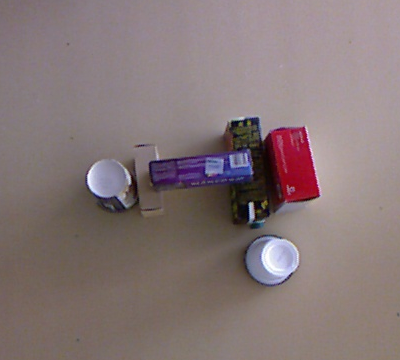
\includegraphics[width=\textwidth]{Img/ObjectSegmentation/seg2_rgb.png}
\end{subfigure}
\begin{subfigure}[t]{0.2\textwidth}
\centering
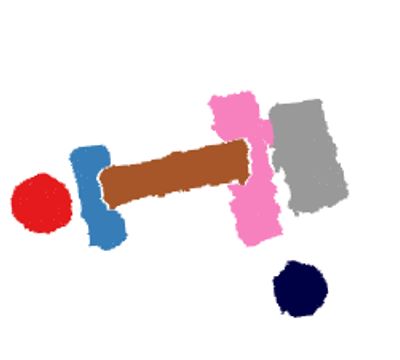
\includegraphics[width=\textwidth]{Img/ObjectSegmentation/seg2.png}
\end{subfigure}
\caption{Example of segmentation results.}\label{fig:seg_results}
\end{figure}

Note that the algorithm works mainly considering geometric properties, and not the color of the pixels. Considering the colors could lead to worst segmentation results for our case of studio since many objects have no only one color.

\begin{wrapfigure}{r}{6.5cm}
\centering
\caption{Box with a green stripe.}\label{fig:seg_color}
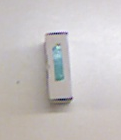
\includegraphics[width=3.5cm]{Img/ObjectSegmentation/color_seg_problem.png}
\end{wrapfigure}
A color based segmentation could segment a draw on an object, or a small part of the object, as a different object, but this, accordingly to the strategy we are going to use (see next sections), would lead to an unfeasible problem. 
For instance, in Figure \ref{fig:seg_color} is shown a box with a green stripe on its top surface, a segmentation algorithm based also on colors could lead to segment the green stripe as another object, and the result is that it is impossible to grasp the green stripe without collide with the box. Vice versa, any interaction with the box is impossible without having a collision with the green stripe. This is the main reason the segmentation we used is based only on geometric features (The \ttt{LCCP} algorithm has the option to include color importance but we neglected it). 

\todo[inline]{Talk about filtering}

\section{Background}
\label{sec:background_alg}
%\begin{itemize}
%\item collison detection
%\item pca
%\item table projection - convex hulls
%\item rotation matrices
%\end{itemize}

In this section will be presented some concepts that will be used to execute the actions and to compute the predicates. 

\paragraph{Principal Components}
The first concept to know is the concept of principal directions. The principal direction of an object is its principal axis which is defined as any of three mutually perpendicular axes about which the moment of inertia of a body is maximum. For instance, for a rectangular object its principal direction is the axis aligned with its longest dimension. 

To obtain the principal axis the principal component analysis (PCA) \citep{PCA} technique is used. This technique is a common statistical procedure that uses orthogonal transformation to convert a set of  observations of possibly correlated variables into a set of values of linearly uncorrelated variables, which are called principal components. The transformation is defined in a manner that the first component has the largest variance, the second has the second largest variance and so on. The principal components are orthogonal because they are the eigenvectors of the covariance matrix, which is symmetric. An example of the principal components for a 2D data set is depicted in Figure \ref{fig:pca1}\footnote{Image taken from \href{https://en.wikipedia.org/wiki/Principal_component_analysis}{https://en.wikipedia.org/wiki/Principal\_component\_analysis}}. The principal components are computed through the covariance matrix of the set of observation, and its eigenvectors $\bar{\lambda_v}$ represent the principal components while its eigenvalues $\lambda$ represent the variance of the data set along the principal component $\bar{\lambda_v}$. 

\begin{figure}[h]
\centering
\begin{subfigure}[t]{0.45\textwidth}
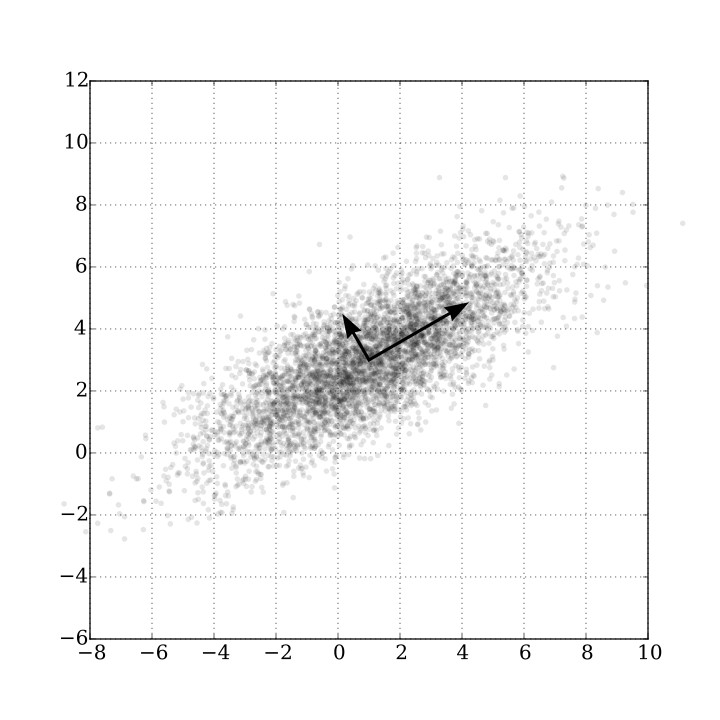
\includegraphics[width=\textwidth]{Img/pca/pca.png}
\caption{}\label{fig:pca1}
\end{subfigure}
\begin{subfigure}[t]{0.45\textwidth}
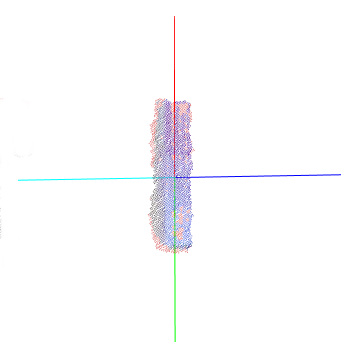
\includegraphics[width=\textwidth]{Img/pca/pca2.png}
\caption{}\label{fig:pca2}
\end{subfigure}
\caption{\textbf{Principal Components Analysis -} In Figure \ref{fig:pca1} PCA for a standard 2D set of observations. In Figure \ref{fig:pca2} results of the PCA for a rectangular segmented object. The \textcolor{green}{green}, \textcolor{red}{red} lines refers to different ways of the first principal components, while \textcolor{blue}{blue} and \textcolor{cyan}{cyan} lines refers to different ways of the second principal directions. The third one would be orthogonal to the first two principal components.}
\end{figure}

A generic point cloud can be seen as a set of observations and the PCA can be directly applied in to the object's point cloud to retrieve its principal components, or how called in this work principal directions. In Figure \ref{fig:pca2} the principal directions of a generic object are illustrated. 

\paragraph{Projection onto a plane}
We will see later that several things need the concept of the projections of a point into a plane. Considering a point $p={x_p,y_p,z_p}$ and a plane $P$ defined by the following equation
\begin{equation}
a x + by + cz + d = 0
\end{equation}
the projection $p_P$ of point $p$ onto the plane $P$ is given by the following set of operations:
\begin{enumerate}
\item Given the origin point $P_0=(x_0,y_0,z_0)$ of the plane, which can be calculated by arbitrary $x_0$ and $y_0$ coordinates as
\[
z_0 = \frac{-1}{c}(ax_0 + by_0 + d),
\]
\item calculate the coordinates of $P_0$ with respect the point $p$
\[
P^{p} = p - P_0,
\]
\item then calculate its projection $\lambda_p$ onto the plane normal $n=(a,b,c)$
\[
\lambda_p = \bar{n} \cdot p^{plane}, 
\]
\item compute the coordinates of the projection onto the plane of point $p$ with respect to the point itself:
\[
p_P^p = - \lambda_p \bar{n}
\]
\item translate it by the coordinate of the points in order to have the projection of the point expressed with respect the original reference frame:
\[
p_P = \bar{p_P}^p + p. 
\]
\end{enumerate}

\paragraph{Rotation Matrices}
Rotation matrices are matrices which express a rotation between two reference frames. Given two frames $\{A\}$ and $\{B\}$, and the rotation matrix $\prescript{A}{B}R$ that defines the rotation of $\{B\}$ relative to $\{A\}$ then a point $\prescript{A}{}P$ with respect frame $\{A\}$ is given by $\prescript{A}{}P=R^{A}_{B}\prescript{B}{}P$, where $\prescript{B}{}P$ is the same point relative frame $\{B\}$. 

Having a desired frame $\{B\}$ defined by axis $\hat{\prescript{A}{}X_B},\hat{\prescript{A}{}Y_B}$ and $\hat{\prescript{A}{}Z_B}B$, where $\hat{\prescript{A}{}Y_B}$ is the y axis of frame $\{B\}$ relative to frame $\{A\}$, the rotation matrix between $\{B\}$ and $\{A\}$ is defined as
\[
R^{A}_{B} = 
\begin{bmatrix}
\hat{\prescript{A}{}X_B} \\
\hat{\prescript{A}{}Y_B} \\
\hat{\prescript{A}{}Z_B} \\
\end{bmatrix}
\]
To transform any object, such as the gripper mesh model, to frame $\{B\}$ then the following homogeneous transform is applied:
\[
H = 
\begin{bmatrix}
R^{B}_{A} & \prescript{A}{}B_O \\
\bar{0} & 1
\end{bmatrix}
\]
where  $R^{B}_{A}={R^{A}_{B}}^{\top}$ and $\prescript{A}{}B_O$ is the origin of frame $\{B\}$ relative to $\{A\}$. In this way, having some axis that defined our new reference frame, we can transform the gripper model in such a way its closing point is in the origin of the new frame and its orientation is the one defined by the new reference frame. 

\paragraph{Axis Aligned Bounding Box (AABB)}
Axis aligned bounding box is a bounding volume defined with respect the reference frame of an object. It is therefore aligned to the objects principal components. A bounding volume is a closed volume that completely contains the object\footnote{\href{https://en.wikipedia.org/wiki/Bounding_volume}{\url{https://en.wikipedia.org/wiki/Bounding\_volume}}}.
After a transformation of the object from its frame and the world frame the dimension of the bounding box are obtained by computing the maximum and minimum coordinates of the point cloud. In this way it is possible to have an approximation of the length, width and height of an object. 

\paragraph{Convex Hull}
A convex hull of a point cloud $P$ is the smallest 3D convex set that contains $P$. 
\begin{figure}[h]
\centering
\begin{subfigure}[t]{0.3\textwidth}
\centering
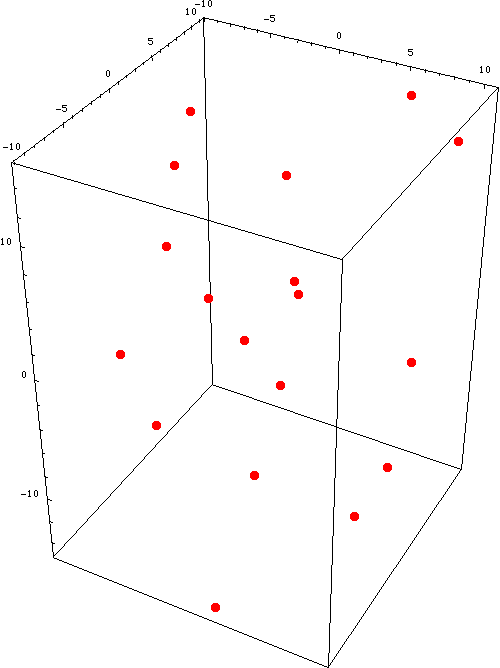
\includegraphics[height=4cm]{Img/convexhull/ch1.png}
\caption{Pointcloud}
\end{subfigure}
\begin{subfigure}[t]{0.3\textwidth}
\centering
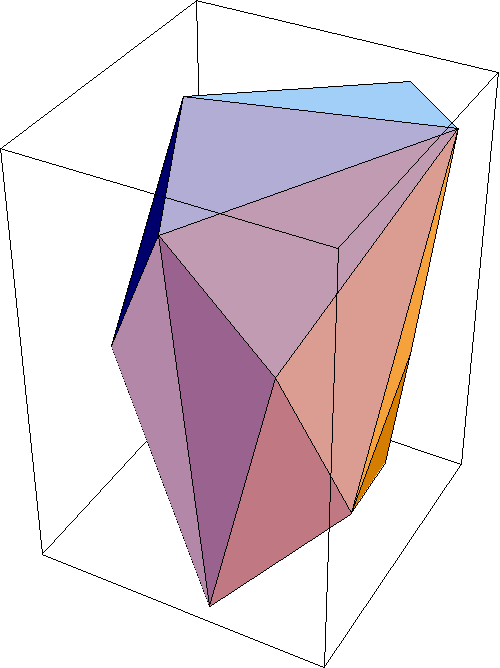
\includegraphics[height=4cm]{Img/convexhull/ch3.png}
\caption{Convex hull}
\end{subfigure}
\caption{Convex hull example}\label{fig:convexhull_example}
\end{figure}
In Figure \ref{fig:convexhull_example} an example of the convex hull for a point cloud is shown. The vertices are first detected and then connected among them by means of triangles. In this way a triangle mesh is associated to the convex hull. 

\paragraph{Collision Detection}
To understand if an object impeds a certain action, such as the pushing along a direction, we have to check if along the desired trajectory the pushed object will collide with a certain one. The collision detection is therefore a crucial step for the predicates computation. There exist different techniques to assert if two objects are colliding, all of them need a representation of the object, which could be for example a basic shape or a more complex as an octree. 

The mesh shape has been thought to use since it can be directly obtained from a \textit{convex hull}. 

Given two objects A and B and their configurations $\bf{q_A}$ and $\bf{q_B}$, the discrete collision query returns a boolean value about whether two objects collide or not. Two objects collide if
\[
A(\bf{q_A}) \cap B(\bf{q_B}) \neq 0
\]

The collision detection will be used to understand if in a given pose $\bf{q}$ the object $A$ will collide with the other objects in the scene.

To make the collision detection most collision libraries, before to use complex algorithm to detect collision between two shapes, they first check if the AABB of the objects intersect, if they don't the objects surely don't collide. If their AABB intersect the objects might collide.

\paragraph{Objects Modelling}
The triangle mesh needed for the collision checking can be directly retrieved by the convex hull. But there is a consideration to take into account. The Kinect, given its pose, is only able to see mainly the top surface of the objects and not all the sides, and therefore we cannot apply directly the convex hull algorithm to the detected surfaces. If we would apply the convex hull on an object's surfaces, we will have likely the situation in which a surface $S$ transformed in a configuration such that it will be above or below another one, and the collision detection will detect no collision since the two surfaces are not colliding. This is because we are totally missing the rest of information about the geometry of the object since we only know the objects surfaces.

\begin{figure}[h]
\centering
\begin{subfigure}[t]{0.3\textwidth}
\centering
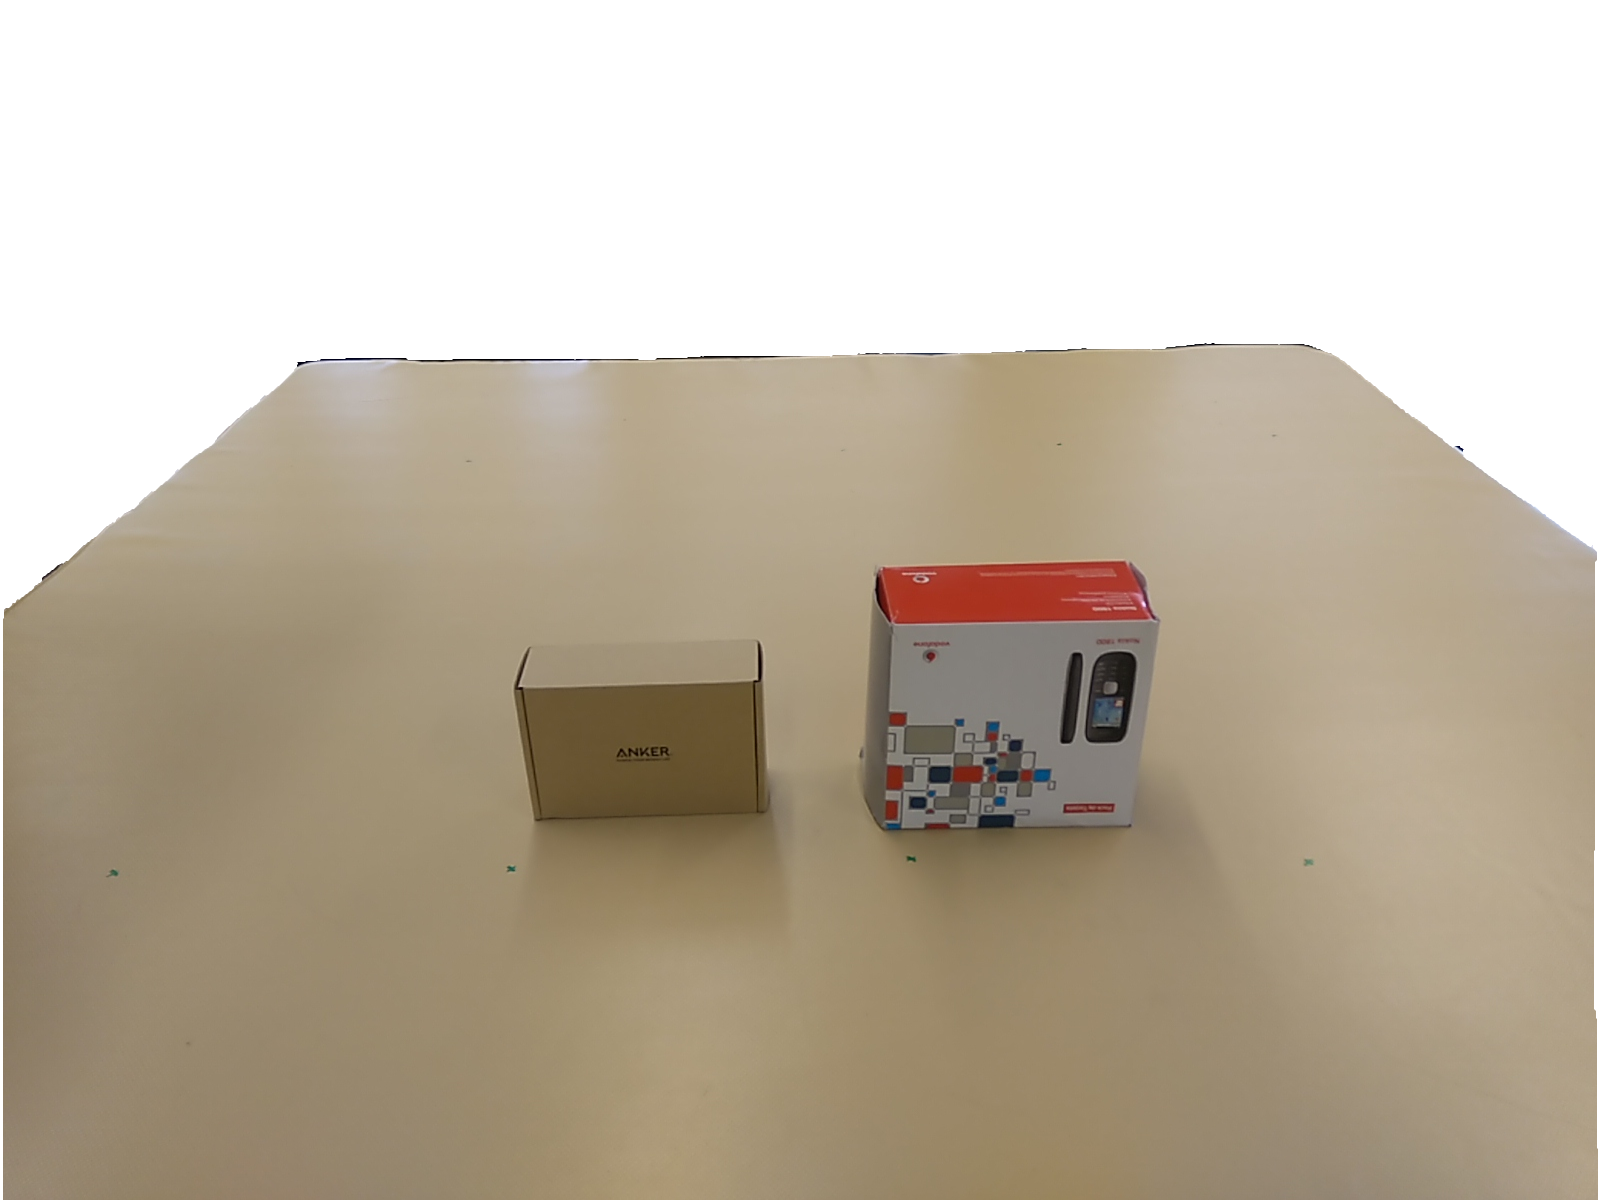
\includegraphics[width=0.9\textwidth]{Img/convexhull/example_only_top_surfaces.png}
\caption{}\label{fig:rgb_top_surfaces_example}
\end{subfigure}
\begin{subfigure}[t]{0.3\textwidth}
\centering
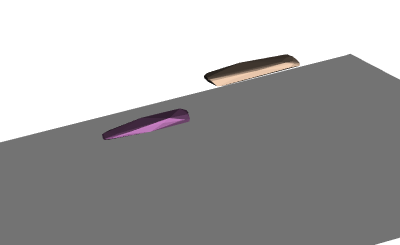
\includegraphics[width=0.9\textwidth]{Img/convexhull/cv_top2.png}
\caption{}\label{fig:cv_top}
\end{subfigure}
\begin{subfigure}[t]{0.3\textwidth}
\centering
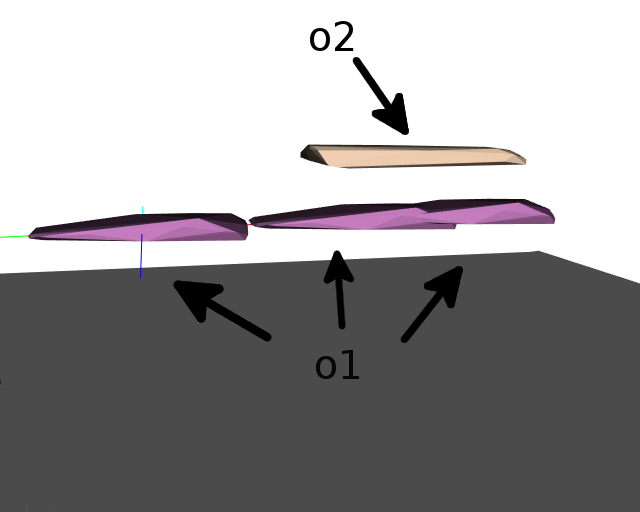
\includegraphics[width=0.9\textwidth]{Img/convexhull/cv_top_collision2.png}
\caption{}\label{fig:cv_top_collision}
\end{subfigure}
\caption{Convex hulls and collision detection using the segmented objects retrieved by the \ttt{LCCP} segmentation algorithm. The gray surface represents the plane's 2D convex hull. In Figure \ref{fig:cv_top} it is possible appreciating that we miss the information about the hidden part of the object. In Figure \ref{fig:cv_top_collision} a collision detection example is depicted. The convex hull is translated along a direction and no collision is detected with any possible translation since the two convex hull will not intersect.}
\end{figure}

From the Kinect's point cloud also the table plane is known, so all the information we have are: the table plane model and the segmented objects (mainly the top surfaces).
If an human would be in the same pose of the Kinect, looking at the table, it will imagine that the objects are not floating surfaces, and he/she will deduce the objects shape from the shape of the top surface. Since in this work we assumed to work with parallelepipeds, the sides of the objects can be easily deduced by projecting the top surface's edges to the plane and then filling the missing object's sides with points. To do that we have to detect the top surface's edges. A more trivial method is directly projecting all the points of the surfaces onto the table plane and then apply the convex hull algorithm to the resulting point cloud given by the sum of the top surface and its projection. In this way the missing sides are indirectly retrieved by the convex hull. 

\begin{figure}[h]
\centering
\begin{subfigure}[t]{0.45\textwidth}
\centering
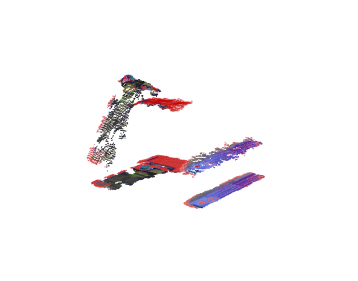
\includegraphics[width=0.9\textwidth]{Img/convexhull/projection.png}
\caption{Surfaces projection}\label{fig:projection}
\end{subfigure}
\begin{subfigure}[t]{0.45\textwidth}
\centering
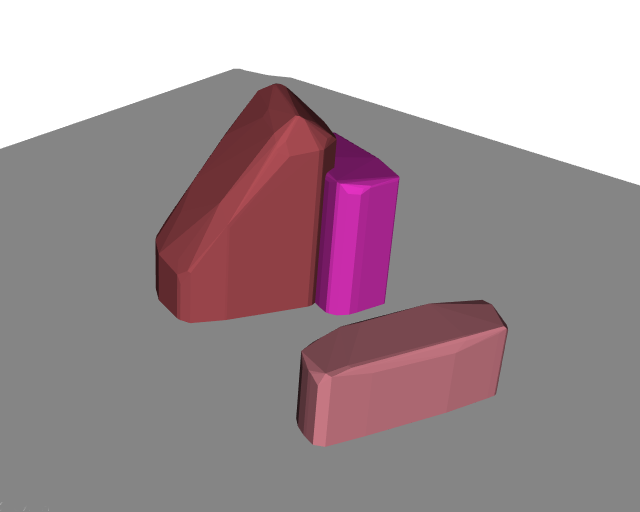
\includegraphics[width=0.9\textwidth]{Img/convexhull/full_convexhull2.png}
\caption{Resulting convex hull}\label{fig:full_convexhull_}
\end{subfigure}
\caption{Convex hull of the objects using their projections onto the table plane.}\label{fig:full_convexhull}
\end{figure}

%The PCL convex hull algorithm returns the convex hull as a triangular mesh, which can be used by the FCL for the collision detection. 

%The pose of the Kinect camera is above the table pointing forward it. In such a pose the Kinect is only able to see mainly the top side of the objects, and not their sides. 
%--- discussed the convex hull relating into to the neccesity for the collision detection.



\section{Actions Execution}
In this section the way the actions are executed is discussed, since the predicates computation depends on the way we decided to execute the actions.  


\subsection{Pushing}
\label{subsec:pushing}

Pushing is a difficult action to execute when the goal is to move one object from one pose to another one. At the best of my knowledge  there are still no methods in state of the art that faced this problem. The majority of pushing actions in object manipulation have the aim to interact with the objects in order to move them and validate the segmentation \citep{katz2014perceiving} \citep{katz2011interactive} \citep{Katz_2013_7407} , without taking care about the final position of the objects. Hermans er al. \citep{conf/iros/HermansRB12} presented a novel algorithm for object singulation through pushing actions, here the pushing actions have the aim to separate objects in cluttered scenes but they are not interested in singulate tidily the objects but just to find a feasible interaction to singulate them. This means that the pushing action could move several objects and the pushing direction is not chosen accordingly the object to push but accordingly to the plane that separate the objects. This results in a pushing action without any guarantee that the pushed objects follows the desired path. Grasping , although is a difficult task, has already an advanced state of the art regarding finding grasping pose also for complex objects. Somehow grasping is easier because it does not consider the whole object geometry but it is focused on looking for local futures that can be interesting for grasping the object (i.e. antipodal points). When we push an object all the object geometry has to be taken into account in order to find a suitable pushing direction. Moreover, humans push objects with a certain initial direction chosen accordingly the object geometry and then adapt the pushing direction accordingly to the error with respect the desired one. This would imply the implementation of a controller which is out the scope of this thesis. 

We are considering to work with objects with simple shapes, such as parallelepipeds. 
A human would push such object mainly accordingly its principal axis and the one orthogonal to its (i.e. the first 2 principal components of Figure \ref{fig:pca2}), but he/she also could push it along the diagonal thanks to the several amount of freedom of the hands. 
Inspired by this consideration, we decided to consider as possible directions to push an object  its first two principal components, the third is orthogonal to the object and it is not of interest for pushing. In particular, there are two senses for each direction, so in total we have 4 possible pushing directions per object, as depicted in Figure \ref{fig:directions}.

\begin{figure}
\centering
\begin{subfigure}[t]{6cm}
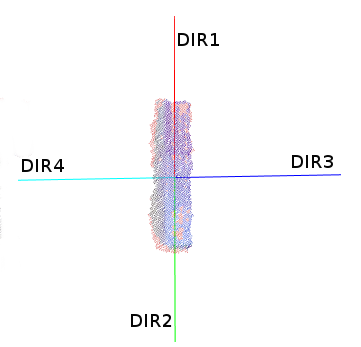
\includegraphics[width=5.5cm]{Img/pushing/directions.png}
\caption{Pushing directions computed using the segmented surface seen by the Kinect.}\label{fig:directions1}
\end{subfigure}
\begin{subfigure}[t]{6cm}
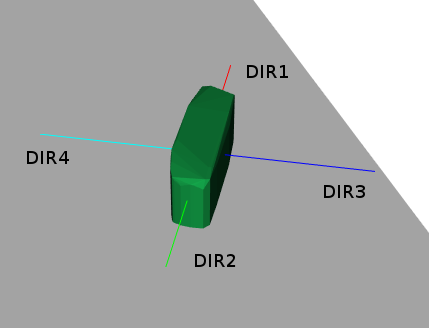
\includegraphics[width=5.5cm]{Img/pushing/directions2.png}
\caption{Pushing directions associated to the object's convex hull.}
\label{fig:directions2}
\end{subfigure}
\caption{Example of pushing directions.}\label{fig:directions}
\end{figure}

Another things to take into account is that the principal directions are not parallel to the table plane. The Kinect could see some sides of the objects, and these sides will affect the direction of the principal components. An object which stands on top of a table will be obviously pushed along a direction parallel to the table. As previously described in Section \ref{sec:background_alg} a point can be projected on to the table plane, but a point and a vector (the principal components are vectors) have the same representation, and therefore we can apply exactly the same equations to obtain the projections of the principal components onto the table plane. So the pushing directions considered are not the one obtained by the PCA but their projections. 


Next, having some pushing directions along with the robot will push the objects, the pose of the end effector (i.e. the gripper) to push the object has to be decided. The pose has been chosen accordingly to the shape of the end effector.
\begin{wrapfigure}{r}{3.5cm}
\centering
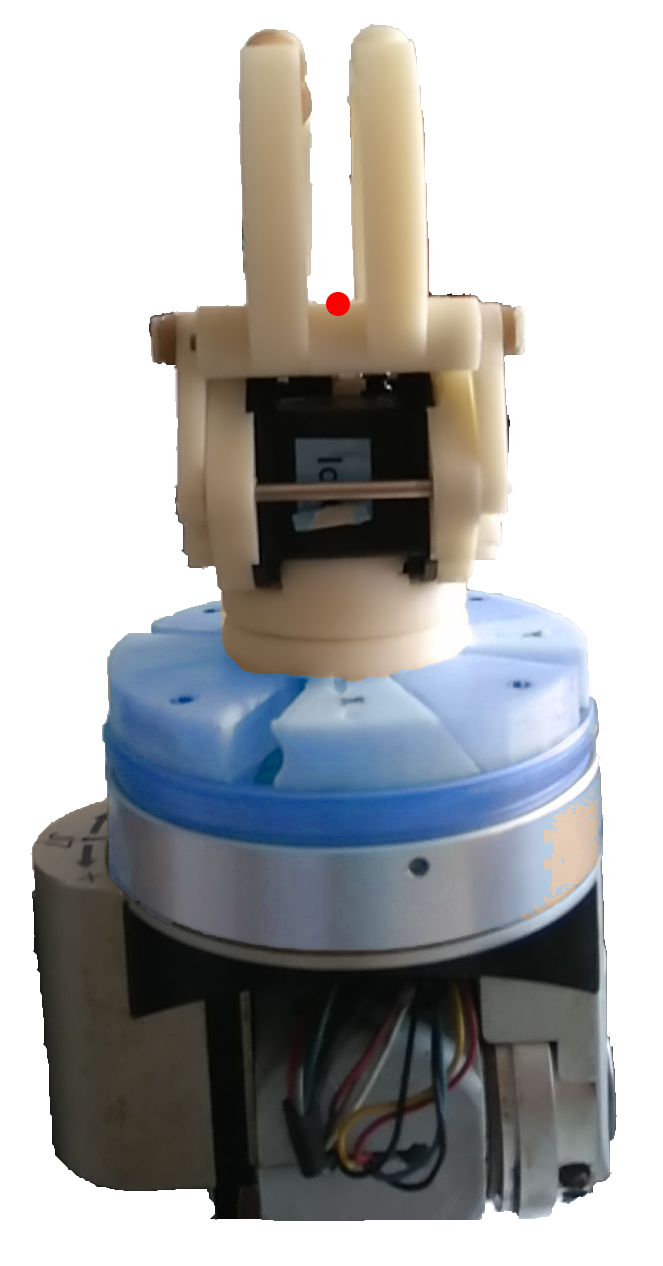
\includegraphics[width=3.5cm]{Img/set_up/gripper_side2.png}
\caption{Gripper's profile view and robot's end effector.}\label{fig:gripper_side}
\end{wrapfigure}
In Figure \ref{fig:gripper_side}
is possible observing the profile of the gripper mounted to the last link of the robot, highlighted by the blue color. Such last link has a circular shape and the gripper's deep is less then the last link. It is undesirable pushing an object with a circular, or spherical, shape for the end effector because there is more probability to make the object no follow the desired path. The gripper has no a circular shape and it is all symmetric, this make it suitable to push an object with a certain stability, i.e. make the object follow the desired path, during the action. As final consideration, we don't want that the last link of the robot touch the objective object since we want a pushing action accurate as most as possible. 

Knowing also the height of the objects retrieved by its AABB, it is possible having a pose for the gripper is such a way that the end effector does not touch the object. The gripper's pose, relative the object, is computed in manner to locate the red point of Figure \ref{fig:gripper_side} to be at the same height of the object. In this way the fingers will fully touch the object during the pushing action. Moreover, to make easy for the robot reaching the pushing pose, it was defined to be a certain distance from the object (in our experiment it was set to 5cm). It would be difficult to reach a pose which is tangent to an object without colliding with it.  

\begin{figure}[h]
\centering
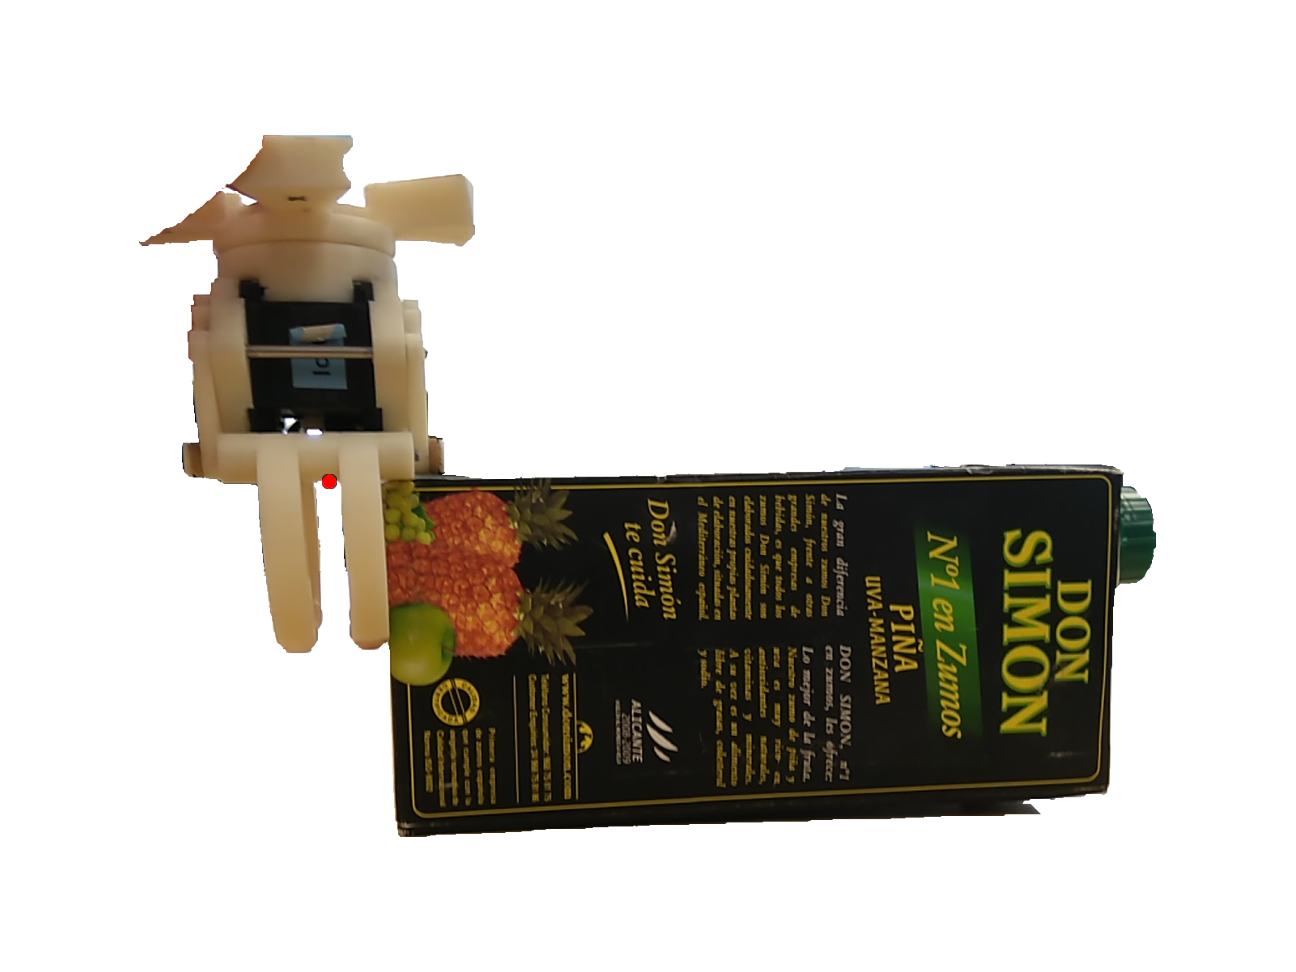
\includegraphics[width=7cm]{Img/pushing/pushing1.png}
\caption{Profile view of a desired pose for pushing an object.}\label{fig:pushing_pose}
\end{figure}

Due to the limited opening width of the gripper (8 centimetres) the object the robot is going to manipulate have small width. This means that when pushing along the principal axis, the object's width is likely small. Such a situation is depicted in Figure \ref{fig:pushing_way1}. Pushing in such a way the gripper will likely push also the black juice box. Therefore when pushing along the principal axis the pose is chosen to be the one in Figure \ref{fig:pushing_way2}. Of course is more stable a pushing pose like the one in Figure \ref{fig:pushing_way1}, since the contacts point (the fingers) are more distant. For this reason that pose is used only when pushing the objects along a direction orthogonal to the principal axis. 


\begin{figure}[h]
\centering
\begin{subfigure}[t]{0.45\textwidth}
\centering
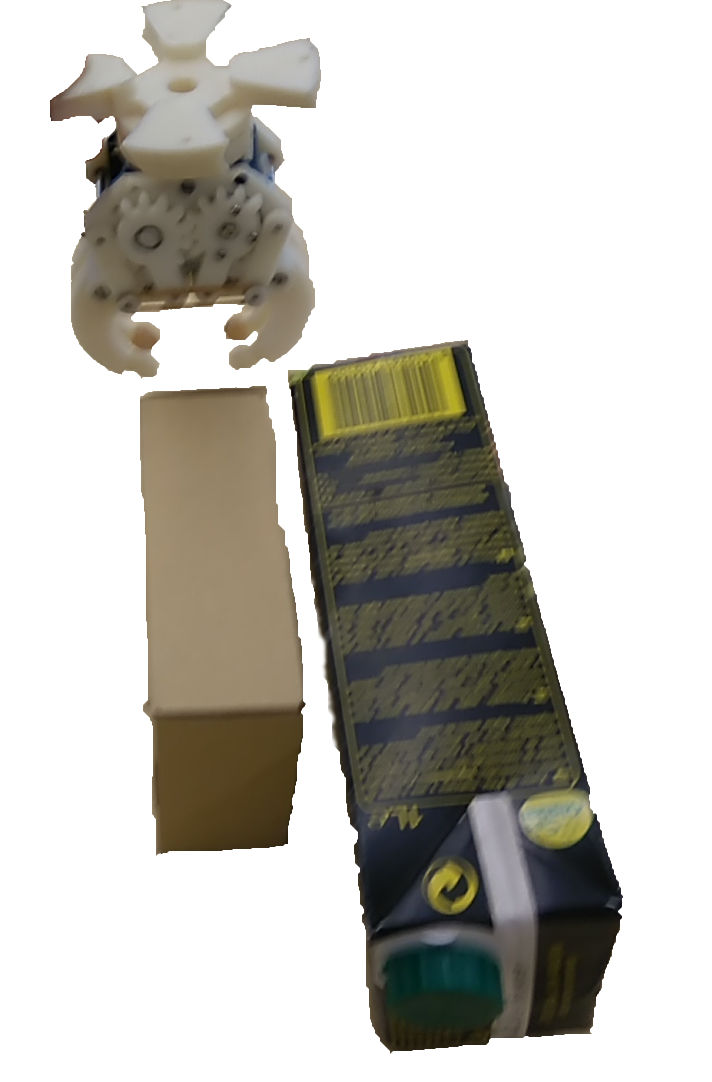
\includegraphics[width=3cm]{Img/pushing/pushing333.png}
\caption{}\label{fig:pushing_way1}
\end{subfigure}
\begin{subfigure}[t]{0.45\textwidth}
\centering
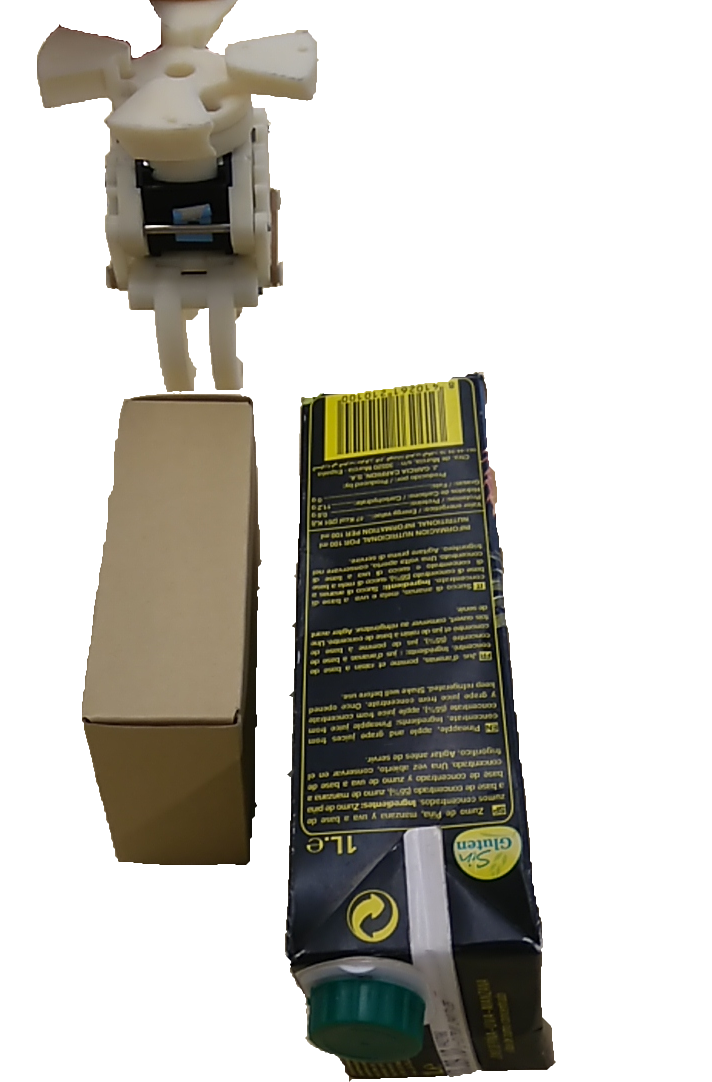
\includegraphics[width=3cm]{Img/pushing/pushing222.png}
\caption{}\label{fig:pushing_way2}
\end{subfigure}
\caption{\textbf{Possible pushing poses for push an object along its principal axis} - In Figure \ref{fig:pushing_way1} the closing direction of the gripper is orthogonal the pushing direction, and for the case depicted in the figure the gripper will likely push also the black juice box. In Figure \ref{fig:pushing_way2} the closing direction of the gripper is parallel to the pushing direction.}\label{fig:pushing_way}
\end{figure}

Having a the projections of the principal components, the table normal and the gripper closing point coordinates it is possible defining a transform defined by the following rotation matrix and translation vector:

\begin{equation}
R_{dir1} =
\begin{bmatrix}
dir2_X & dir2_Y & dir2_Z \\
dir4_X & dir4_Y & dir4_Z \\
n_x & n_y & n_z \\
\end{bmatrix}^{\top}
\qquad \qquad
T=
\begin{bmatrix}
c_x \\ c_y \\ c_z
\end{bmatrix}
\label{eq:transform}
\end{equation}
where $dir1_X$ refers to the x coordinate of the vector that defines the direction 1, $n$ is the table normal and $c$ is the desired tool central point. Eq. \ref{eq:transform} refers for a pushing along direction 1, where the gripper's closing direction has to be parallel to the pushing direction. The rotation matrix $R_{dir3}$ for pushing along direction 3 would be the same of $R_{dir1}$. 

As previously said, the planner consider to push the objects at infinity, in reality the robot has to push the objects for a finite length. Since the planner has no geometric information, the pushing length is chosen accordingly the dimension of the AABB relative to the pushing direction. For instance, if the robot is going to push the object $1$ along direction 1 the length $l$ of the pushing action is $l=k \cdot AABB_1.length$, where $k$ is a gain factor (1 in our experiments) called \textit{pushing step}. This is a big limitation since the robot will push an object accordingly to the manipulated objects, not to surrounding ones. 

The first pose is the pushing pose while the last pose is the pushing pose translated along the pushing direction by the length of the push. To retrieve the path the we consider the total length and we discretize it by $n$ points having in this way $n+2$ poses (2 because of the pushing pose and the final pose). For each pose the inverse kinematic is done. In this way we obtain a discrete path. 

When the robot approaches the pushing pose it could be that it collides with other objects. It would be suitable to use \textit{MoveIt!} which can built an octomap representation of the scene and find a path avoiding collision with the scene. Although this technique is very powerful and correct for this application is quite time consuming. We avoid this by simply considering a pre pushing pose which has the same pose of the pushing pose but translated, accordingly the table normal, $10$ centimetres from the pushing pose. 
After the execution of the pushing action the robot goes to its \textit{home} pose (depicted in Figure \ref{fig:setup_}) in order not to fall inside the Kinect's view. When it goes to home it might happen that it collides with some objects, so also for the final pose with consider another one translated, accordingly the table normal, $10$ centimetres from the last pose. 
In this way the pushing trajectory is defined by a total of $n+4$ poses. 


%Note that we can obtain with this method is:
%\begin{itemize}
%\item pushing direction for simple objects: we can push the rectangular object of Figure \ref{fig:pca2} along one of the ways of the first two principal directions, 
%\item assign a reference frame to the object: by using the three principal components we can obtain a new reference frame $F_{o_i}$ for each object.
%\end{itemize}

%The computed principal components are orthogonal between themselves but the way of eigenvector $\bar{\lambda}$ is chosen by the PCA algorithm. In our case we are interested having a coherent description of the pushing directions as indicated in Figure \ref{fig:pca2}, and for that aim $\bar{\lambda_2}$ has to be always the same way with respect to the first principal component $\bar{\lambda_1}$. 

\subsection{Grasping}
\label{sec:grasping}
%\todo[inline]{Review of grasping techniques}
%\textbf{ROS object\_manipulator}\\

There exist an advanced state of the art regarding grasping. Despite this all the techniques of grasping are very computationally expensive. Many of them rely on the identification of the shape of the objects and then a set of pre-built grasping poses is returned and they can be very robust as the method proposed by Brook et al. \citep{brook2011collaborative}. Other techniques rely on the identification of local features which can state if a grasping pose is feasible or not. Two very goods grasping planning algorithms, which deal with novel objects, published past year are AGILE \citep{AGILE} and HAF \citep{haf}, despite this how shown in \citep{covallero} they are not so robust and they are computationally expensive and not suitable for this thesis. In order to have a faster planning algorithm we considered a very simple approach to grasp the objects, which is suitable only with the kind objects we are going to interact with. Despite this the planner present by this thesis can be directly integrated (with just few modifications) with several grasping algorithms. 

The idea is to grasp the object in manner that the gripper's closing direction is orthogonal the principal axis of the object. The approaching direction of the gripper is given by the third principal component of the object. Then the gripper also is centred accordingly the centroid of the object. 
In this manner a single grasping pose is obtained for each object. 

\todo[inline]{Add exactly how the gripper position is computed}

To grasp the object also the robot needs a pre grasping pose, if not the gripper will collide with object attempting to reach the grasping pose, moving it away, and the grasp will fail. The pre grasping pose is simply defined by the grasping pose translated along its approaching vector by $10$ centimetres.

The grasping action, in its total is composed by the following set of actions: 
\begin{enumerate}
\item Reach the pre grasping pose
\item Open gripper
\item Reach grasping pose
\item Close gripper
\item Reach pre grasping pose again: this is done in order to avoid collisions between the grasped object and the other ones
\item Go to the dropping pose: the object will be dropped into a bin
\end{enumerate}

\section{Predicates Computations}
In Chapter \ref{ch:planning_system}  the predicates used are described, in this section their computation is presented in detail. 

Once the objects have been segmented, we have one point cloud per object, next we have to retrieve the symbolic predicates from the objects configuration. 

\subsection{Predicate: \texttt{block\_grasp}}
The \ttt{block\_grasp o1 o2} predicate refers the fact that object \ttt{o1} impedes \ttt{o2} to be grasped. The computation is this predicate is straightforward: the mesh model of the opened gripper is transformed to the grasping pose of object \ttt{o2}, and check if it collides with the other objects. In figure \ref{fig:block_grasp} such procedure is shown and in Algorithm \ref{alg:block_grasp} the pseudo algorithm is described in detail. 

\begin{figure}[h]
\centering
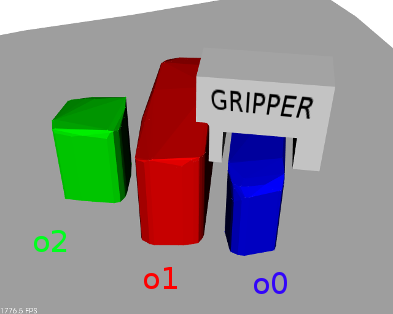
\includegraphics[width=6.5cm]{Img/grasping/block_grasp.png}
\caption{Visualization of the computation of \texttt{block\_grasp} predicate for object \ttt{o0}. The opened gripped model is transformed to the grasping pose for object \ttt{o0} and it is tested if the gripper mesh model collides with the other objects, in this case it collides with \ttt{o1}. }\label{fig:block_grasp}
\end{figure}

\begin{algorithm}
\caption{Computation of \texttt{block\_grasp} predicate. $O$ is the set of objects (convex hull retrieved with the projection onto the table plane) and $G_{poses}$ is the set of grasping poses of all the objects.}\label{alg:block_grasp}
\begin{algorithmic}
\Function{ComputeBlockGraspPredicates}{$O$,$G_{poses}$}
  \texttt{block\_grasp\_predicates} = \textsc{NULL}
\ForAll{$A = objects \in O$}
  \State $openGripperMesh \gets$ \textsc{trasnformGripperModel}($G_{poses}(A)$)
\ForAll{$B = objects \in O$}
  \If{$A \neq B$} 
	\State $collision \gets$ \textsc{isThereCollision($openGripperMesh$,$B$)}
	\If{collision}
		\State \texttt{block\_grasp\_predicates} = \textsc{AddPredicate}(\texttt{block\_grasp B A})
	\EndIf
  \EndIf
\EndFor
\EndFor \\
\Return  \texttt{block\_grasp\_predicates}
\EndFunction
\end{algorithmic}
\end{algorithm}   
 
Notice that this method implies to check for collision between the gripper and objects that might be very far from the interested object, i.e. there is no need to compute the collision detection.  Despite this, how explained in Section \ref{sec:background_alg} the most collision detection algorithm first check if the AABB of the objects intersect. This is a computationally cheap operation, and only if their AABB intersect the computationally expensive algorithm are used to check for collision. This makes the Algorithm \ref{alg:block_grasp} efficient and computationally not expensive. It has been observed that, in average, to compute this predicate the time is about $8$ milliseconds. This for two main reason, the objects are far between each other and their AABB do not intersect, or in case they intersect the gripper mesh model is relatively simple compared to the convex hull of an object, this makes the collision detection algorithm faster because it has to check for the intersection of less triangles. 
 
\subsection{Predicate: \texttt{on}}
The \ttt{(on o0 o1)} predicate means that object \ttt{o0} is on top of object \ttt{o1}. With the convex hull of the objects is easy to understand if two objects are one on top of the other on by checking for collision, but in this way we do not know who is above and who is below. To do this their surface projections onto the table plane are used. 
The research group of Artificial Intelligence and Robotics Laboratory of
Istanbul Technical University, published some interesting researches suitable to the aim of this thesis. In \citep{ersen2014scene} \citep{SSS147762} \citep{ersen2013extracting} the authors proposed some approaches to enhance
 3D recognition and segmentation results to create and maintain a consistent world model involving attributes of the objects and spatial relations among them. Their researched focused on modelling the world for manipulation planning tasks. They do not consider scene like the one of this thesis but simpler ones such as  a pile of cubes above each other. What can be directly used from their work is the computation of the \ttt{on} predicate. The \textit{on} relation for a pair of objects is determined by checking whether their projections on the table plane overlap. This predicate was not a relevant part of their work and they did not provide to much information about its computation. Therefore our implementation for the \ttt{on} predicate is based on their idea with some modifications. 
 
Our idea is based on the fact that an object which stands on top of another one occludes some parts of the object below. While the one below does no occlude any part of the top object. 
Let's consider the scene in Figure \ref{fig:on_predicate_original}, the object \ttt{o0} occludes some parts of object \ttt{o1}. The projections ${\sc P_{0}}$ and ${\sc P_{1}}$ onto the table plane of \ttt{o0} and \ttt{o1} are respectively the red and green ones in Figure \ref{fig:on_1}. This means that the convex hull ${\sc C_{P_{1}}}$ of the projection \ttt{o1} intersect with the projection ${\sc P_{0}}$ of \ttt{o0}, while the projection ${\sc P_{1}}$ of \ttt{o1} does not interesct with the convex hull ${\sc C_{P_{0}}}$ of the projection of \ttt{o0} (Figures \ref{fig:on_2} and \ref{fig:on_3}). 


\begin{figure}[h]
\centering
\begin{subfigure}[t]{0.45\textwidth}
\centering
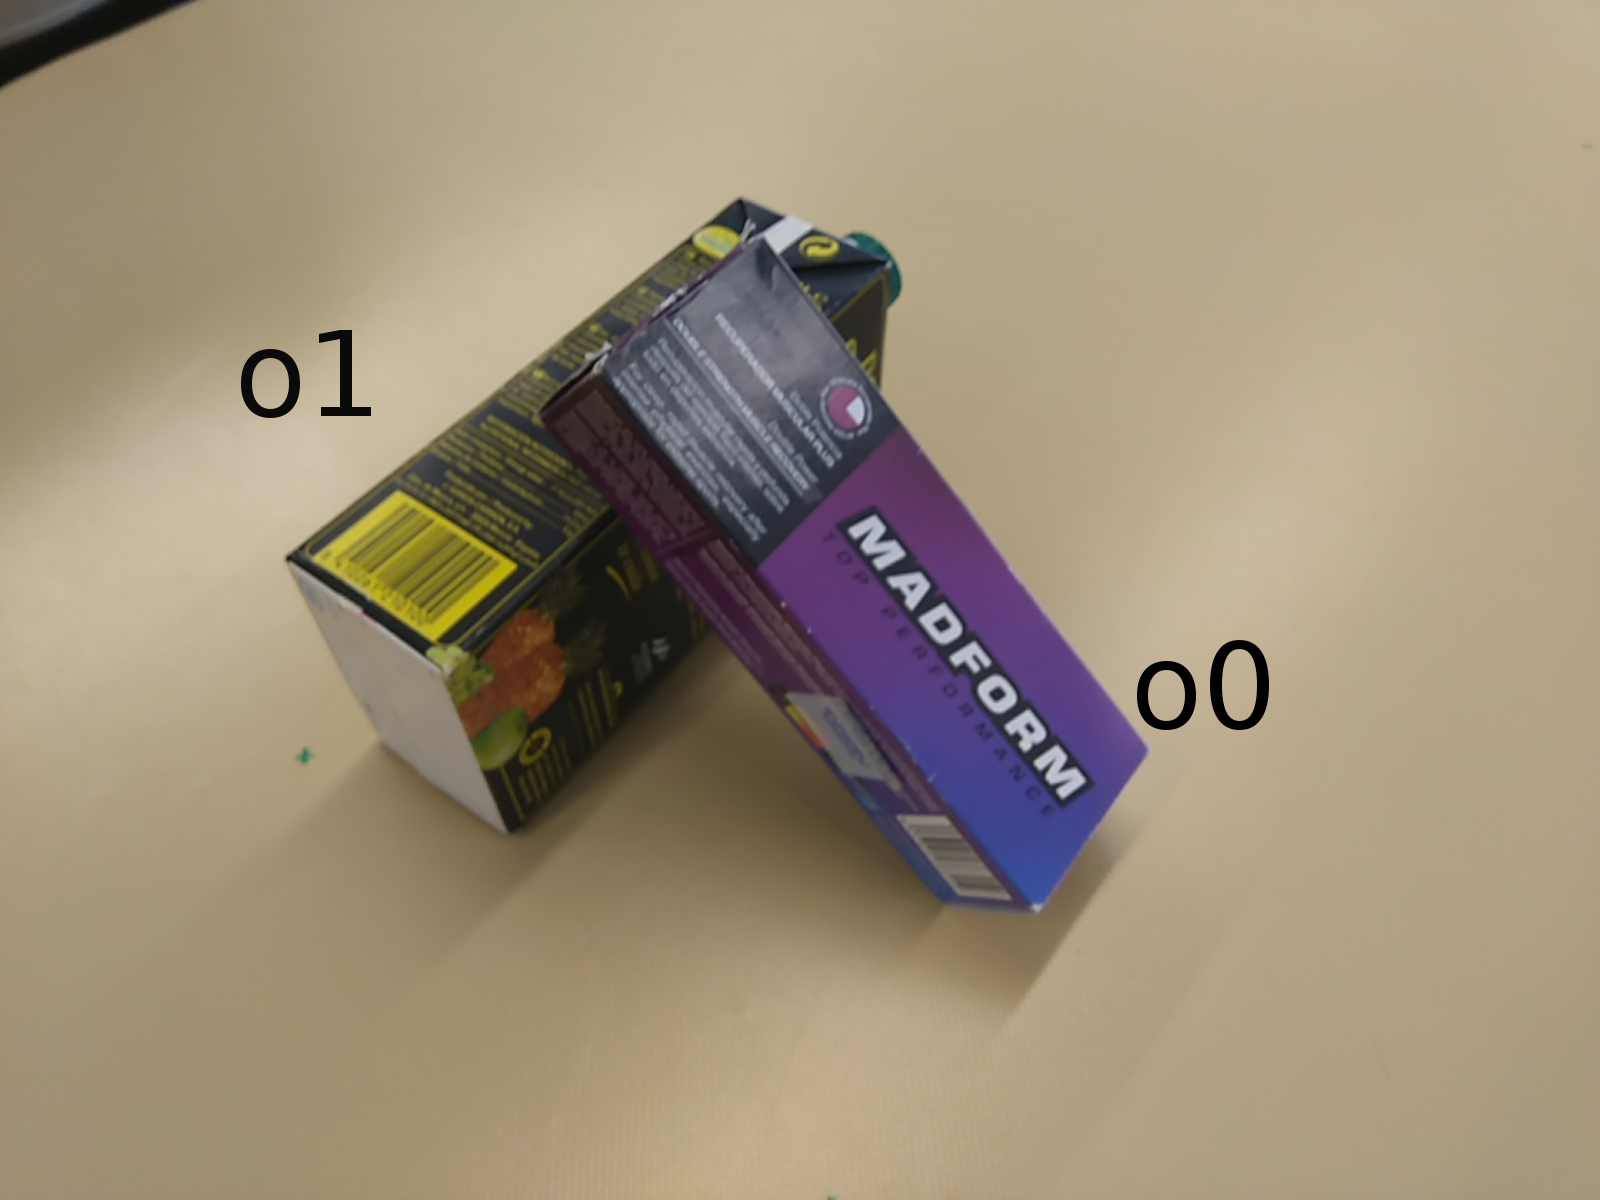
\includegraphics[width=5cm]{Img/on/on1.jpg}
\caption{Scene}\label{fig:on_predicate_original}
\end{subfigure}
\begin{subfigure}[t]{0.45\textwidth}
\centering
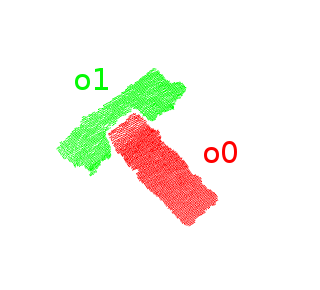
\includegraphics[width=5cm]{Img/on/on2.png}
\caption{$P_0 \quad \& \quad P_1$}\label{fig:on_1}
\end{subfigure}
\begin{subfigure}[t]{0.45\textwidth}
\centering
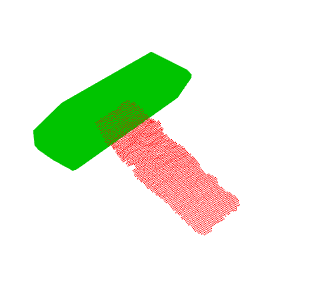
\includegraphics[width=5cm]{Img/on/on4.png}
\caption{${\sc C_{P_{1}}} \quad \& \quad {\sc P_{0}}$}\label{fig:on_2}
\end{subfigure}
\begin{subfigure}[t]{0.45\textwidth}
\centering
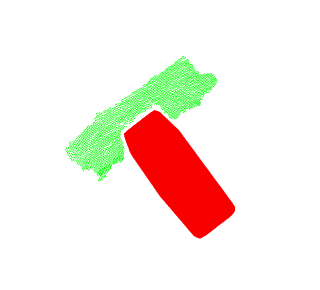
\includegraphics[width=5cm]{Img/on/on3.png}
\caption{${\sc C_{P_{0}}} \quad \& \quad {\sc P_{1}}$}\label{fig:on_3}
\end{subfigure}
\caption{Visualization of the computation of the \ttt{on} predicate. Figure \ref{fig:on_1} show the real image, Figure \ref{fig:on_1} shows the projections of the objects onto the table plan while Figures \ref{fig:on_2} and \ref{fig:on_3} represent the two step strategy to compute the \ttt{on} predicate.}\label{fig:on_predicate}
\end{figure}

Although this method works fine to compute the \ttt{on} predicate it has the limitation that its scope is only for objects for a rectangular shaper. An object that has a form of L has a convex hull that includes big free areas where an object could lie. 

It is important to take into account also that actually the edges of the occluded parts of the below object, once projected, could be at the same position, of some projected edges of the top object. This could be dangerous for the computation of this predicate. Therefore a threshold is added. Focusing the attention on Figure \ref{fig:on_2} it can be appreciated that the intersection ${\sc C_{P_{0}}} \cap {\sc P_{1}}$ has several points, while in case the two edges relative to the occluded and occluding part have similar coordinates, the intersection ${\sc C_{P_{1}}} \cap {\sc P_{0}}$ would have just few points. Therefore the \ttt{(on o0 o1)} predicate is update accordingly to the following mathematical formula:
\begin{equation}
\ttt{(on o0 o1)} =
\begin{cases}
{\sc True}, \qquad length({\sc C_{P_{0}}} \cap {\sc P_{1}}) > th_0 \;\; \wedge \;\; length({\sc C_{P_{1}}} \cap {\sc P_{0}}) < th_1 \\
{\sc False}, \qquad otherwise
\end{cases}
\label{eq:on}
\end{equation}
where $length(A)$ means the number of elements in the set $A$.
The values of the thresholds $th_0$ and $th_1$ are determined empirically and they are $th_0=th_1=100$.

The formula \ref{eq:on} is then evaluated for every possible combinations of objects, that is $n(n-1)$ times, where $n$ is the number of objects. Despite this, its computation is very fast. For the example in Figure \ref{fig:on_predicate} its was evaluated just 2 times since there are only 2 objects and it took $3$ milliseconds, that is $\approx 1.5 \frac{ms}{pair \; of \; object}$. For instance, for a complex scene with 10 objects the total time devoted to compute this predicate would be $10 \cdot 9 \cdot 1.5 \approx 135 ms$ (the $\approx$ symbol is due to the fact that the computation time depends on the number of points of the objects and the complexity of their convex hulls).



\subsection{Predicate: \texttt{block\_dir$_i$}}
The \ttt{(block\_dir$_i$ o1 o0)} predicate, if true, means that object \ttt{o1} impedes object \ttt{o0} to be moved along its $i$-th direction. 

Object \ttt{o1} can impedes object \ttt{o0} to be moved along a certain direction if a collision will appear between the two objects. In order to do that, having a certain pushing length $l_i$ for the $i$-th direction of object \ttt{o0}, its ocnvex hull $C_0$ is translated along the considered direction until reach its final position which is $p_f=p_i + l \cdot dir_i$, where $p_f$ and $p_i$ are respectively the centroid at the final and initial pose. Object \ttt{o0} is going to do a path from its initial and final pose so the collision should be checked along its path. 
To do that we could use a continuous collision detection algorithm or a discrete one. The continuous method suppose that given an object, its initial, its final pose and the other objects in the environment it will detect a collision if a collision occurs from the initial to the final pose. This algorithm has the advantage to be accurate but we should repeat it separately for each object sine we are not interested to see if there is a collision, but we are interested in knowing what is the object it is going to collide with. We decided therefore to use the discrete strategy, that is we consider several poses between the initial one and the final one, including the final one, and for each check if it collides with the other objects. 



\begin{figure}[h]
\centering
\begin{subfigure}[t]{5cm}
\centering
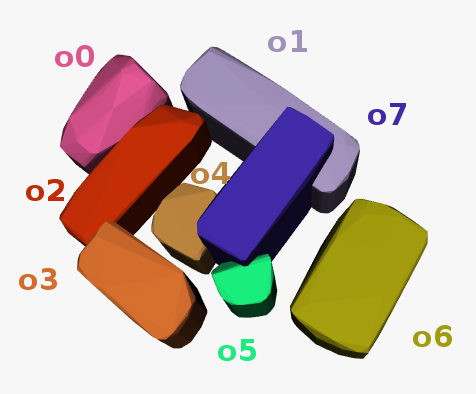
\includegraphics[width=5cm]{Img/block_dir/original_labels2.png}
\caption{Top view of the convex hull of the segmented objects.}\label{fig:block_dir_original}
\end{subfigure}
\begin{subfigure}[t]{5cm}
\centering
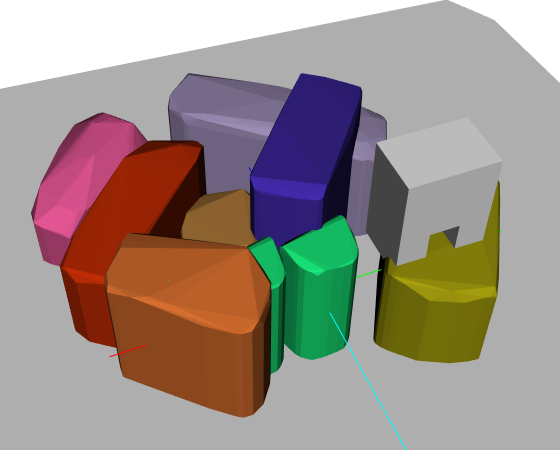
\includegraphics[width=5cm]{Img/block_dir/pushing11.png}
\caption{Evaluating the \ttt{(block\_dir1 * o5)} predicate}\label{fig:block_dir_push1}
\end{subfigure}
\begin{subfigure}[t]{5cm}
\centering
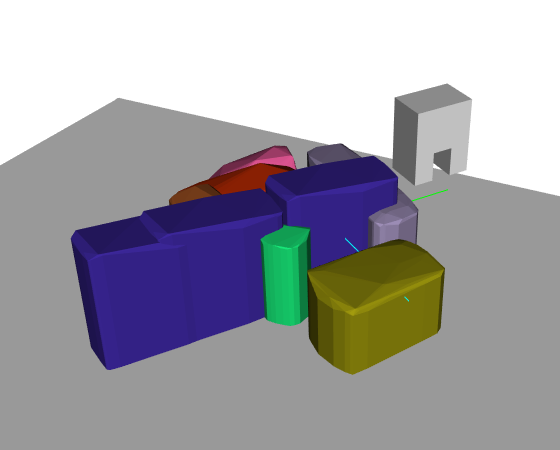
\includegraphics[width=5cm]{Img/block_dir/pushing22.png}
\caption{Evaluating the \ttt{(block\_dir1 * o7)} predicate}\label{fig:block_dir_original}
\end{subfigure}
\begin{subfigure}[t]{5cm}
\centering
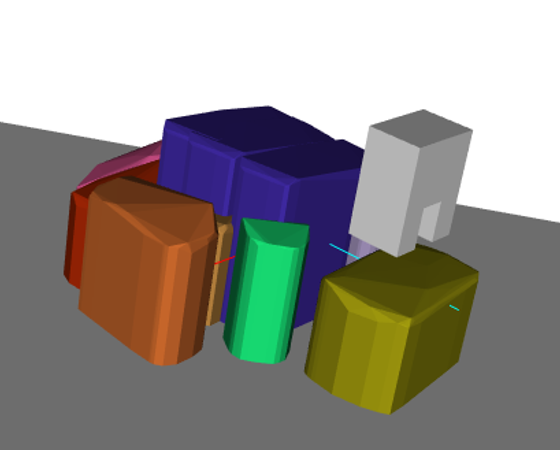
\includegraphics[width=5cm]{Img/block_dir/pushing33.png}
\caption{Evaluating the \ttt{(block\_dir3 * o7)} predicate}\label{fig:block_dir_original}
\end{subfigure}
\begin{subfigure}[t]{5cm}
\centering
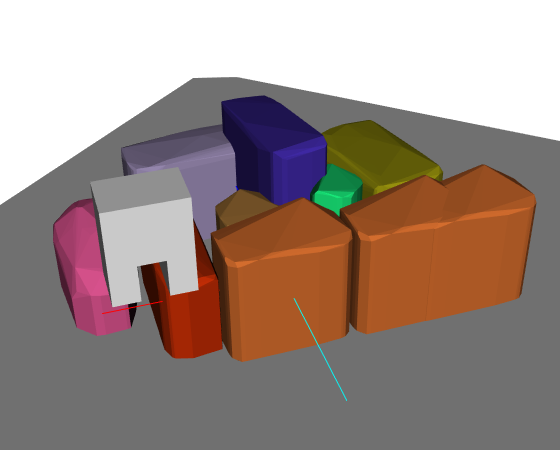
\includegraphics[width=5cm]{Img/block_dir/pushing44.png}
\caption{Evaluating the \ttt{(block\_dir2 * o3)} predicate}\label{fig:block_dir_original}
\end{subfigure}
\begin{subfigure}[t]{5cm}
\centering
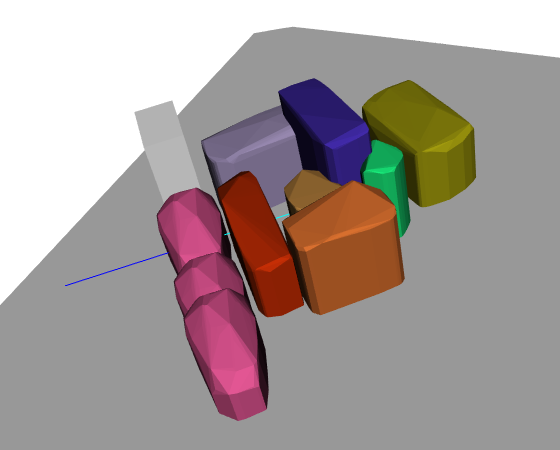
\includegraphics[width=5cm]{Img/block_dir/pushing55.png}
\caption{Evaluating the \ttt{(block\_dir1 * o0)} predicate}\label{fig:block_dir_original}
\end{subfigure}
\caption{Visualization of the computation of \ttt{block\_dir$_i$} predicates. "Evualuating the \ttt{(block\_dir1 * o0)}" means that the algorithm is evaluating for all the objects, except \ttt{o0}, if they collide with \ttt{o0} when pushed along direction 1.}\label{fig:block_dir}
\end{figure}

Considering the kind of objects we are going to interact with, the discrete path  is computed by translating the object along the pushing direction by a length equal to the AABB dimension associated to that direction, until reaching the final pose. Note that no collision detection is done for the object at its initial pose, therefore the total number of poses considered for the pushing path are $n_{poses} = \ceil*{\frac{k \cdot AABB_{dimension}}{AABB_{dimension}}} = \ceil*{k}$, where $k$ is the pushing step defined in Section \ref{subsec:pushing}.

To push an object along a certain direction the robot needs to put its end effector at the opposite side of the object. Therefore object \ttt{o1} can impedes object {o0} to be moved along a certain direction also in the case the end effector cannot be put in the pushing pose because it would collide with \ttt{o1}. This computation is simply done by transforming the closed gripper mesh model to the pushing pose relative the desired pushing direction of the object to push and check for collision with the other objects, as similarly done for the computation of the \ttt{block\_grasp} predicate.

In Figure \ref{fig:block_dir} is shown graphically the procedure to compute the predicate. 


Note that also the gripper during the pushing action will move, so ideally the collision checking should be done exactly how done for the object. We decided to neglect this and check only for the initial pose in order to relax the planner and not to make it too much conservative. This means that during the pushing action the robot might actually move more than one object. Despite this relaxing strategy the algorithm showed to work perfectly and cases in which the gripper moved more than one object were really rare, at least with the objects we used in our experiments. 

\begin{algorithm}[h]
\caption{Computation of \texttt{block\_dir} predicates. $O$ is the set of objects (convex hull retrieved with the projection onto the table plane), $P_d$ is the set of the pushing directions of all the objects, $P_{poses}$ is the set of the initial pushing pose of all the object and $P_{path}$ is the set of all the pushing poses realtive to each direction and each object.}\label{alg:block_dir}
\begin{algorithmic}
\Function{ComputeBlockDirPredicates}{$O$,$P_d$,$P_{poses}$,$P_{path}$}\\
\texttt{block\_dir\_predicates} $\gets$ \textsc{NULL}
\ForAll{$A = object \in O$}
\ForAll{$d = directions \in P_d(A)$}
\ForAll{$p = poses \in P_{path}(A,d)$}
\ForAll{$B = object \in O$}
  \State $A_T \gets$ {\sc transformObject($A,p$)}
  \If{$A \neq B$} 
	\State $collision \gets$ \textsc{isThereCollision($A_T$,$B$)}
	\If{collision}
		\State \texttt{block\_dir\_predicates} $\gets$ \textsc{AddPredicate}(\texttt{block\_dir B A})
	\EndIf
  \EndIf
  \EndFor 
  \EndFor

  \State $closedGripperMesh \gets$ \textsc{trasnformClosedGripperModel}($P_{poses}(A,d)$)
\ForAll{$B = object \in O$}
\If{$A \neq B$} 
	\State $collision \gets$ \textsc{isThereCollision($closedGripperMesh$,$B$)}
	\If{collision}
		\State \texttt{block\_dir\_predicates} $\gets$ \textsc{AddPredicate}(\texttt{block\_dir B A})
	\EndIf
  \EndIf
  \EndFor
\EndFor 
\EndFor \\
\Return  \texttt{block\_dir\_predicates}
\EndFunction
\end{algorithmic}
\end{algorithm}  

The computation of this predicate can be appreciated in detail in Algorithm \ref{alg:block_dir}. From that pseudo code can be noted that the complexity of this function to compute the predicate approximatively is $\mathcal{O}(n \cdot n_{directions} \cdot n_{poses}\cdot (n-1) + (n-1)\cdot n_{directions} )$. 

The computation of this algorithm is the most computational expensive of all the planner since it involves many collision detection phases. In fact the time required to compute this predicate for the example in Figure \ref{fig:block_dir} (considering to push the objects $1.5$ times the AABB dimension relative to the pushing direction) was $\approx 1.115 seconds$, were $\approx 0.869s$ were dedicated to check if the objects will collide when move, while $\approx 0.239s$ were dedicated if the gripper collides with some objects.  

